%!TEX root = ../thesis.tex

\section{A family of graphs not $\emph{k}$-sided for any $\emph{k}$}
\thispagestyle{plain}
  \label{s:fix}
  In this section we prove the following theorem.

  \begin{thrm}
    \label{fix:th:family}
      There is a family of graphs $G_k$ that, for any $k \in \N$, has members that are not $k$-sided.
  \end{thrm}

  As is noted in the introduction all members of this family contain separating $4$-cycles. The maximum vertex degree $d$ of $G_k$ is about $2k+O(1)$. This also means that in principle it might be possible to create an algorithm providing $O(d)$-sided layouts for any corner assignment. Let us repeat that our algorithm in Section~\ref{s:algo} only solves this for corner assignments without separating $4$-cycles.

  \begin{wrapfigure}[16]{r}{6cm}
    \centering
    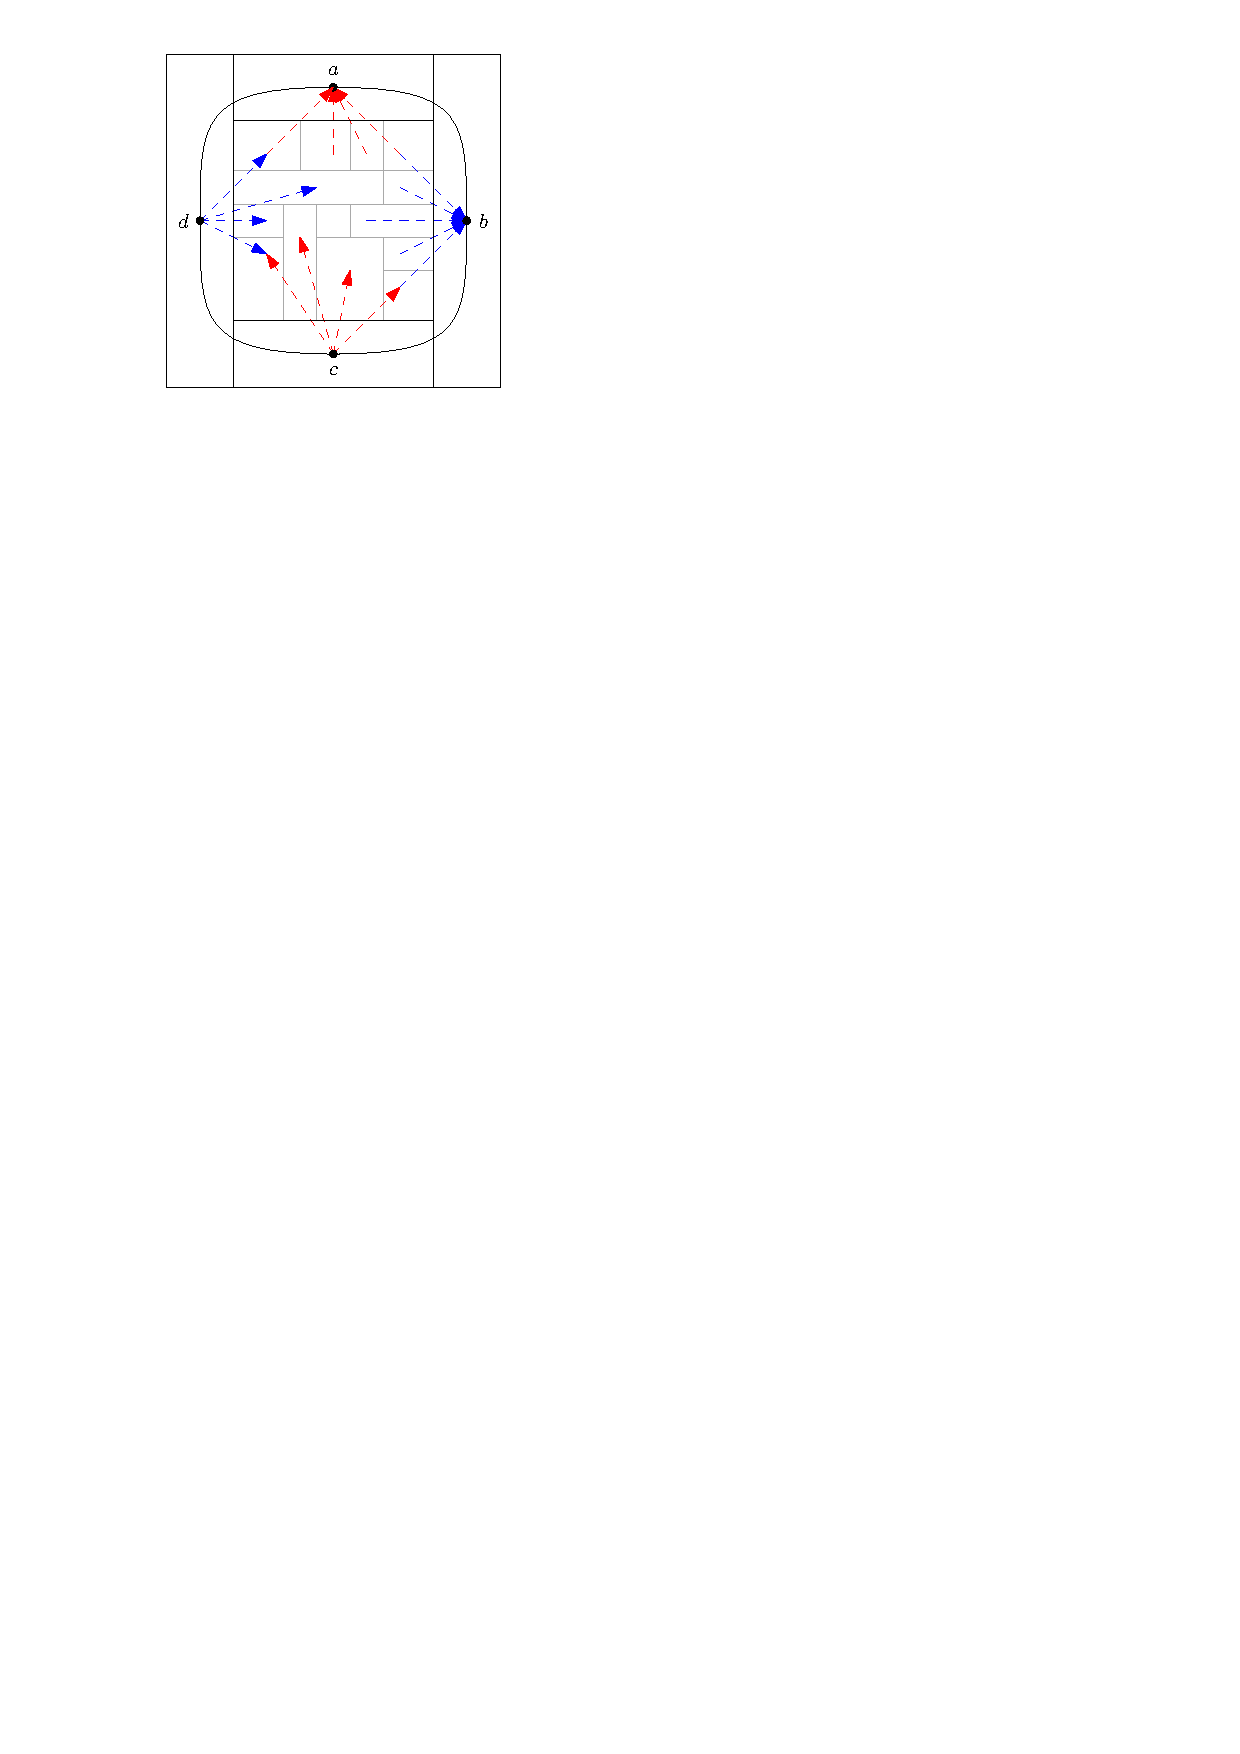
\includegraphics[width=5cm]{fixExtension/img/sep4cycle.pdf}
    \caption{The structure inside a separating $4$-cycle.}
    \label{fig:fix:sep4cycle}
  \end{wrapfigure}

  \mypar{Multiple corner assignments}
  If there is no $k$-sided rectangular dual for a certain corner assignment $\ext G$ of $G$. There may still be another corner assignment of $G$ that admits a $k$-sided dual.
  However, if we use $ H_k = \ext G_k$ as an auxiliary graph we note that $G_k$ is the interior of a separating $4$-cycle of $H_k$. This auxiliary graph will be known as \emph{scaffold} of $G_k$.
  We prove in Lemma \ref{lm:fix:fourCycleInteriorColor} this implies that $G_k$, as induced subgraph, has to be colored in accordance with the corner assignment $\ext G_k$.
  We first have to prove Lemma \ref{lm:fix:fourCycleInteriorColor} before we can prove Theorem \ref{fix:th:family}.

  \begin{lemma}
    \label{lm:fix:fourCycleInteriorColor}
    Let $\C$ be a separating $4$-cycle of $\ext G$ with interior $\I$. We can label the vertices of $I$ by $a$, $b$, $c$ and $d$ in clockwise order such that all interior edges incident to $a, b, c$ and $d$ are incoming red, incoming blue, outgoing red and outgoing blue, respectively.
  \end{lemma}
  \begin{proof}
    The interior $I$ of $\C$ is represented by some rectilinear shape in every rectangular dual $\L$ of $\ext G$. Such a shape must have at least $4$ clockwise right turns if we travel along its boundary in a clockwise direction otherwise the shape is not closed.

    Yet, such a clockwise turn can not occur due to a single rectangle. Instead, such a turn can only occur when two rectangles are adjacent to each other. Because a $4$-cycle represents only $4$ pairs of adjacent rectangles, the representation of $I$ in $\L$ can only have $4$ clockwise turns. Hence, it must be a rectangle, the only rectilinear shape with just $4$ clockwise turns.

    The interior $I$ of $\C$ is represented by a rectangle $\I$ in any rectangular dual. Since two disjoint rectangles can only be adjacent to each other at one side, $\I$ has four sides that need to be covered and $\I$ is adjacent to only four rectangles we know that every side of the rectangle $\I$ is adjacent to a single rectangle. We then denote by $a$ the vertex corresponding to the rectangle above $\I$, $b$ the rectangle right of $\I$, $c$ the rectangle below $\I$ and $d$ the rectangle left of $\I$.
    The construction at the end of the proof can also be seen in Figure~\ref{fig:fix:sep4cycle}.

    Then the required coloring follows from how a regular edge labeling is obtained from a layout.
  \end{proof}

  Hence, if we know the color and orientation of one interior edge incident to a vertex of a separating $4$-cycle $\C$ we know the color and orientation of all interior edges of $\C$ incident to $\C$.

  \begin{wraptable}{R}{6cm}
    \centering
    \begin{tabular}{c|| c c c c}
      $NE$ & $N$ & $ E$ & $ SE$ & $ NW$ \\
      $SE$ & $S$ & $ E$ & $ NE$ & $ SW$\\
      $SW$ & $S$ & $ W$ & $ SE$ & $ NW$\\
      $NW$ & $N$ & $ W$ & $ NE$ & $ SW$\\
    \end{tabular}
    \caption{The neighbors of the new poles.}
    \label{tab:scaffold}
  \end{wraptable}

  Lemma \ref{lm:fix:fourCycleInteriorColor} is useful because it allows us to consider a single corner assignment $\ext G$ of $G$ by using is as scaffold. Suppose we want to investigate some specific corner assignment $\ext G$ of $G$ with poles $N$, $E$, $S$ and $W$ then we can consider the graph $\ext G = H$ as a graph in its own right, and inspect the coloring of this graph.
  $H$ admits a corner assignment $\ext H$ without separating triangles by connecting the new poles as indicated in Table \ref{tab:scaffold}.
  $\ext H$ is shown in Figure \ref{fig:scafold}.
  $G$ is displayed in thick lines and with filled vertices.
  An arbitrary corner assignment $\ext G =H$ is then drawn with thin lines and hollow vertices.
  A corner assignment of $H$ is then drawn with dashed edges and hollow vertices.

  \begin{figure}[t]
  \centering
  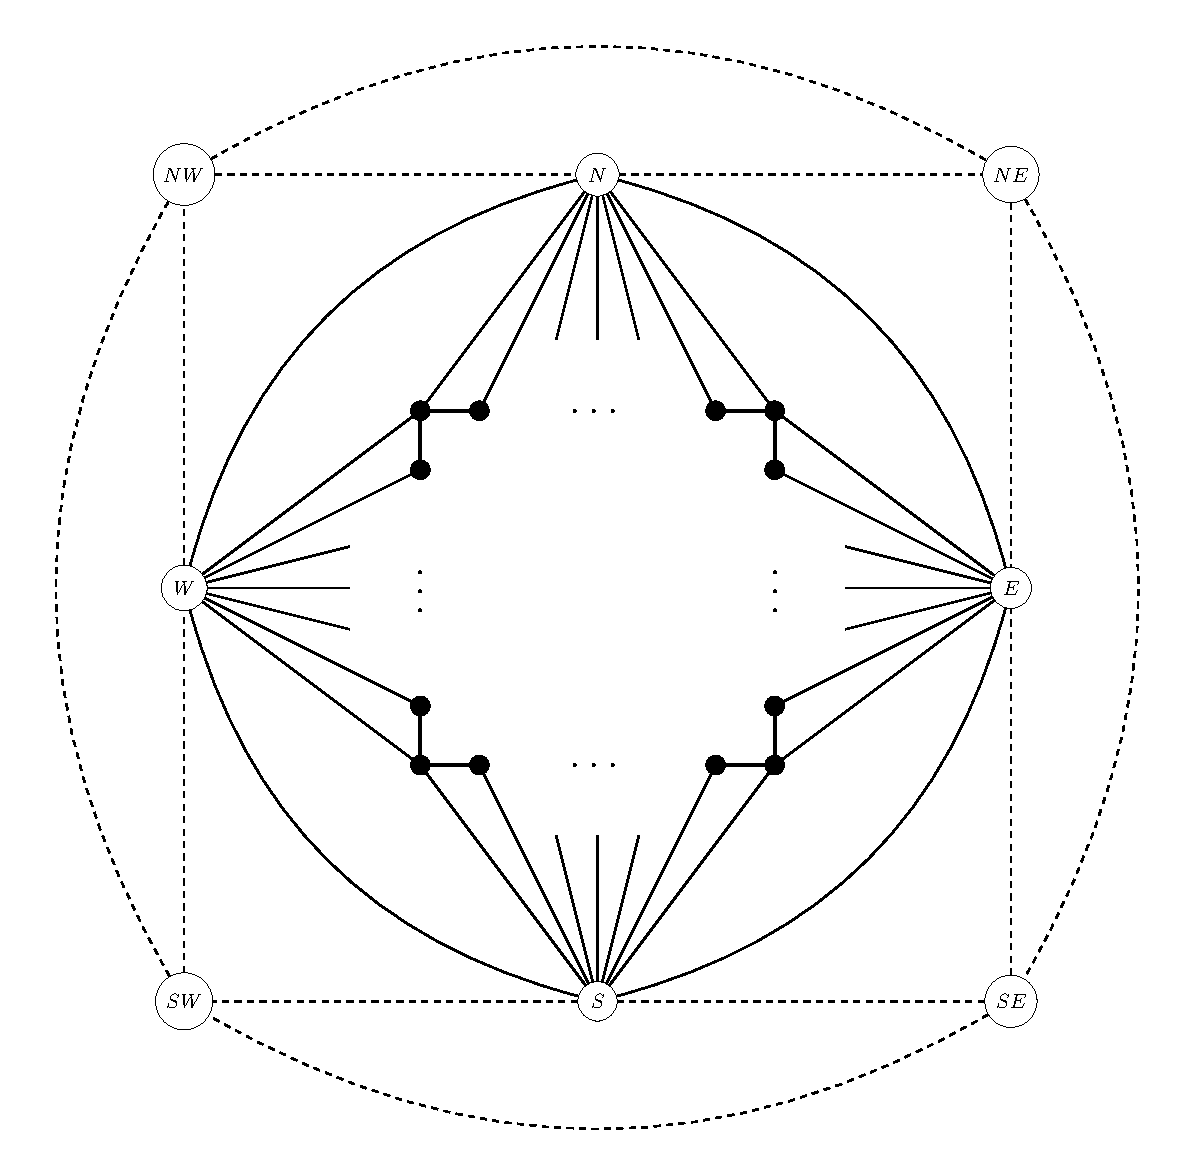
\includegraphics[scale=0.5]{fixExtension/img/scafold}

  \caption{The construction of a scaffold.
      \label{fig:scafold}}
  \end{figure}


  The graph $H$ can have more than one corner assignment but they all contain the separating $4$-cycle $\C= NESW$. Thus, by Lemma \ref{lm:fix:fourCycleInteriorColor} we see that, without loss of generality, the interior edges of $\C$ incident to $N$ are colored incoming red, those incident to $E$ are colored incoming blue, those incident to $s$ are colored outgoing red and those incident to $W$ are colored outgoing blue.

\begin{proof}[Proof of Theorem \ref{fix:th:family}]
  Now as all the preparations are done, we can consider the family of graphs $G_k$ with the corner assignment $\ext G_k$ given in Figure \ref{fig:fix:manymany0}.
  We know we only have to look at this corner assignment since we can force it using a scaffold and Lemma \ref{lm:fix:fourCycleInteriorColor}.
  In $G_1$ the dots are replaced by a single vertex, in $G_2$ the dots are replaced by two vertices and so on.
  Each member has 2 maximal separating $4$-cycles.
  These are both marked by thick lines in Figure \ref{fig:fix:manymany0}.
  Many of the edges in this graph have only one possible color and orientation that does not violate the constraints of a regular edge labeling.
  Firstly, we can color the edges incident with the poles in accordance with the exterior vertex condition.
  Subsequently, we can use Lemma \ref{lm:fix:fourCycleInteriorColor} on both maximal separating $4$-cyles in accordance to color even more edges and finally we can color the edges in triangles of which the other two edges have  the same color using Observation \ref{obs:rel:noMonoColoredTriangles}.
  These forced colorings are performed in Figure \ref{fig:fix:coloring}.

  \begin{figure}[t]
    \centering
    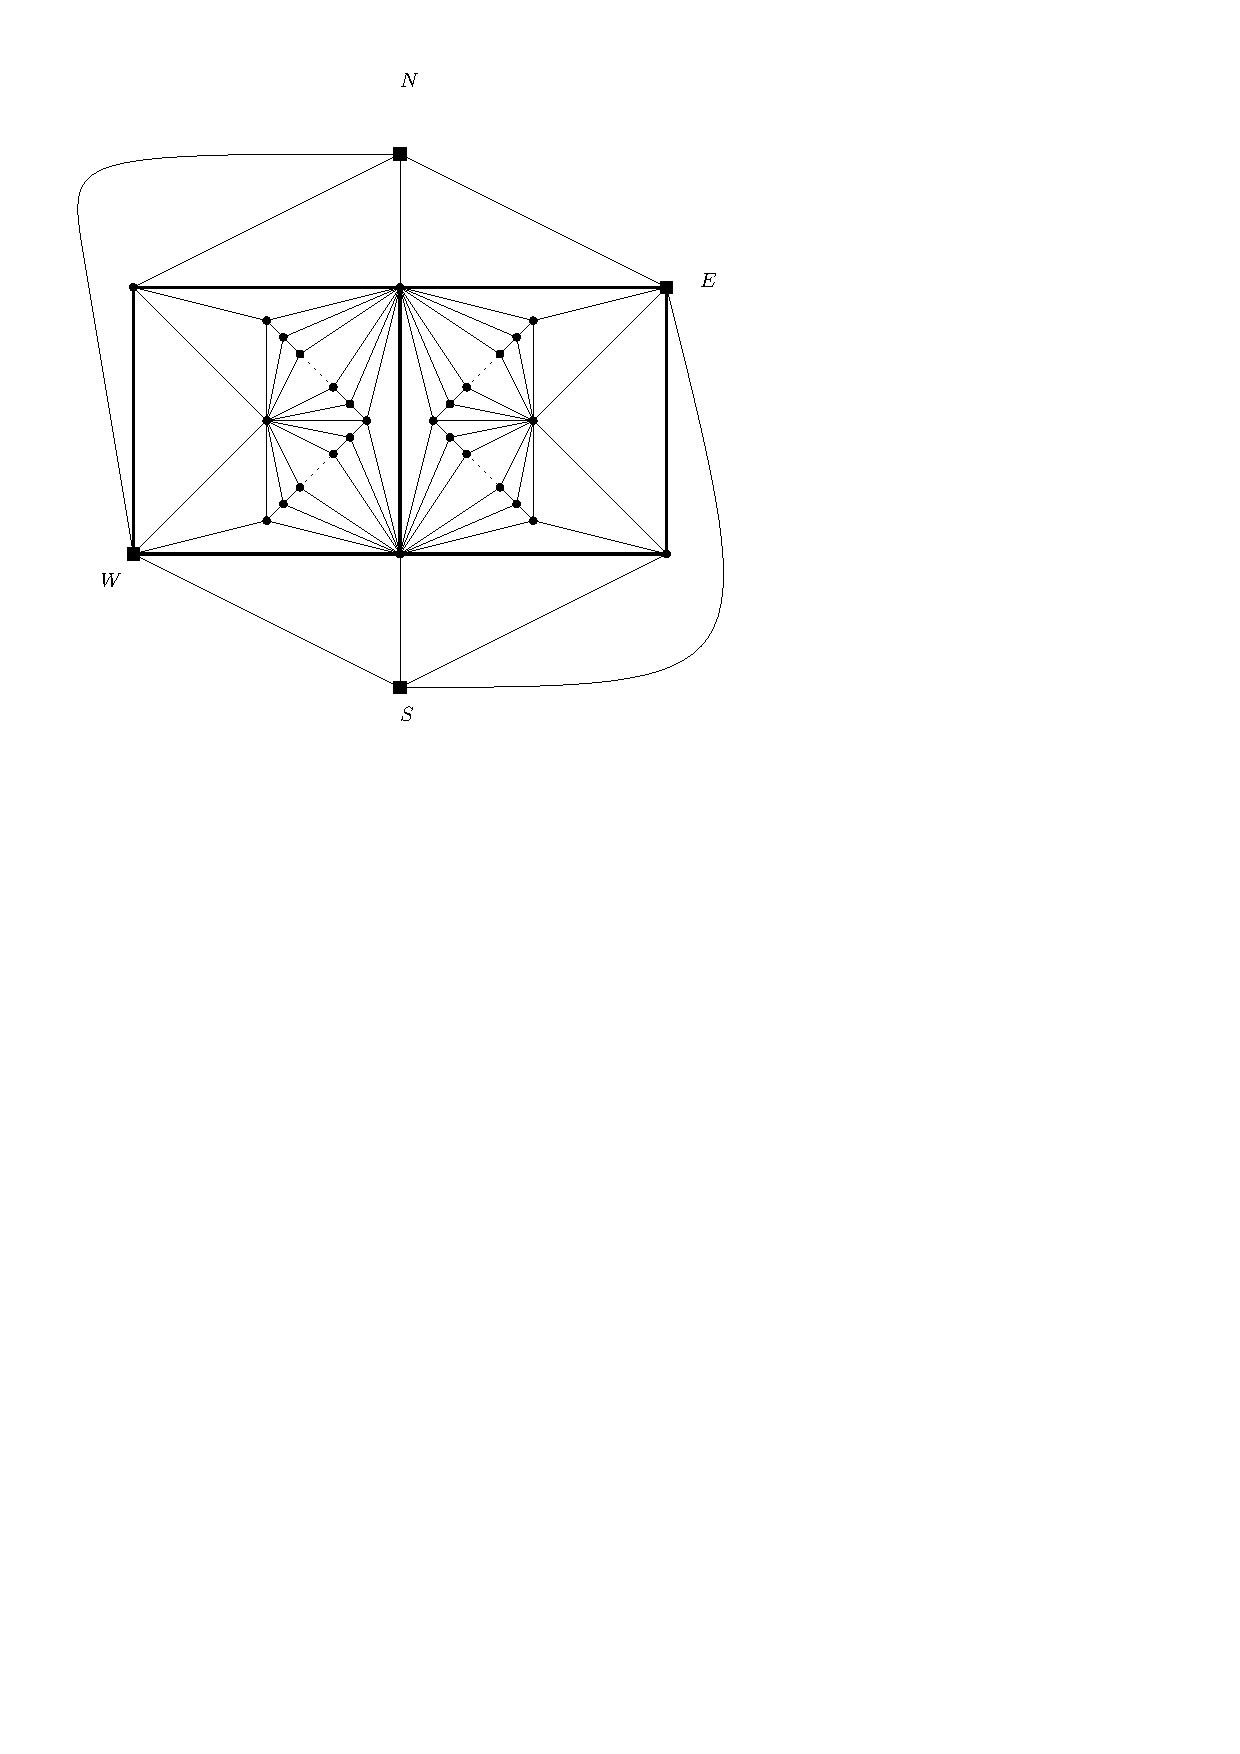
\includegraphics[scale=1]{fixExtension/img/manymanybase}
    \caption{A family of graphs not $k$-sided for any $k$}
    \label{fig:fix:manymany0}
  \end{figure}

  \begin{figure}[h]
    \centering
    \begin{subfigure}[t]{0.3\textwidth}
      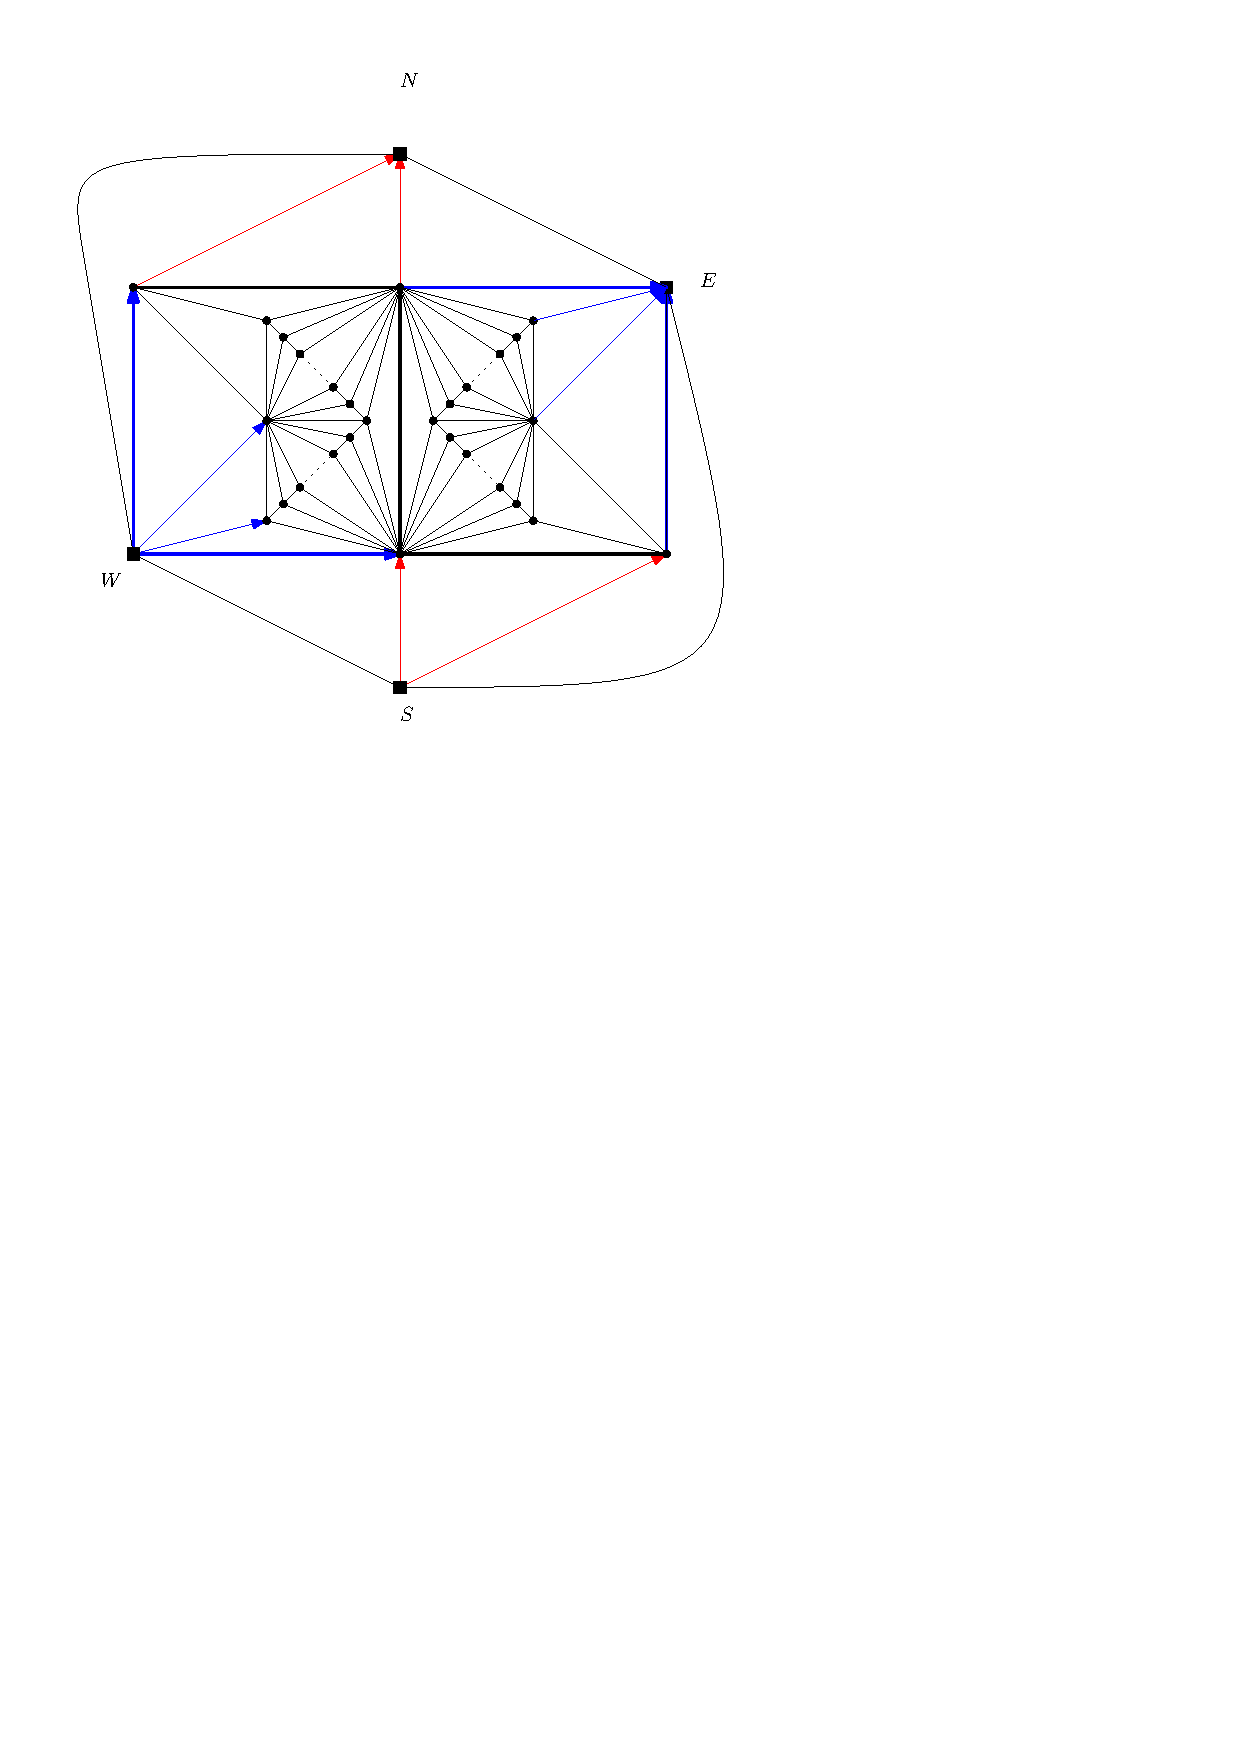
\includegraphics[width=\textwidth]{fixExtension/img/manymany1}
      \caption{Coloring the edges adjacent to the poles.}
      \label{fig:fix:manymany1}
    \end{subfigure}
    \quad
    \begin{subfigure}[t]{0.3\textwidth}
      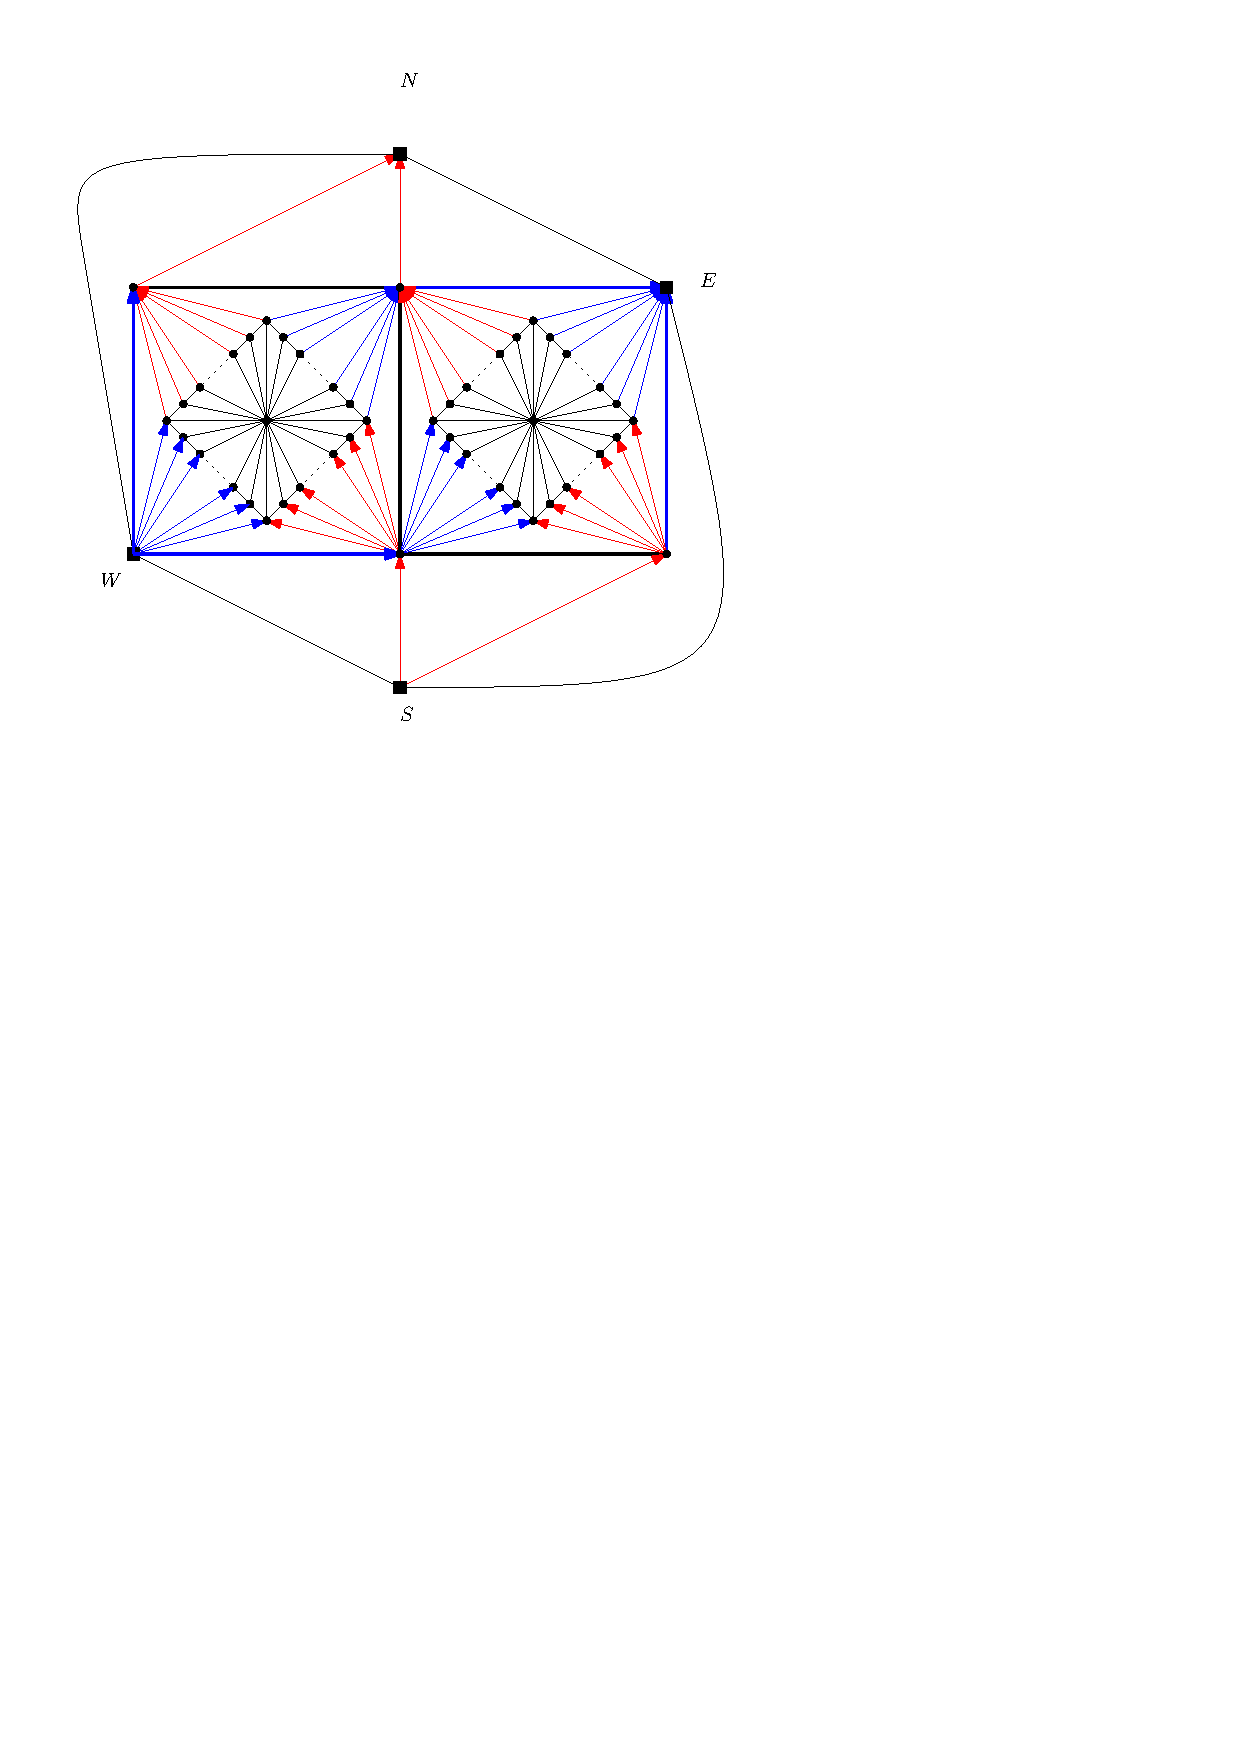
\includegraphics[width=\textwidth]{fixExtension/img/manymany2}
      \caption{Propagate trough the separating $4$-cycle.}
      \label{fig:fix:manymany2}
    \end{subfigure}
    \quad
    \begin{subfigure}[t]{0.3\textwidth}
      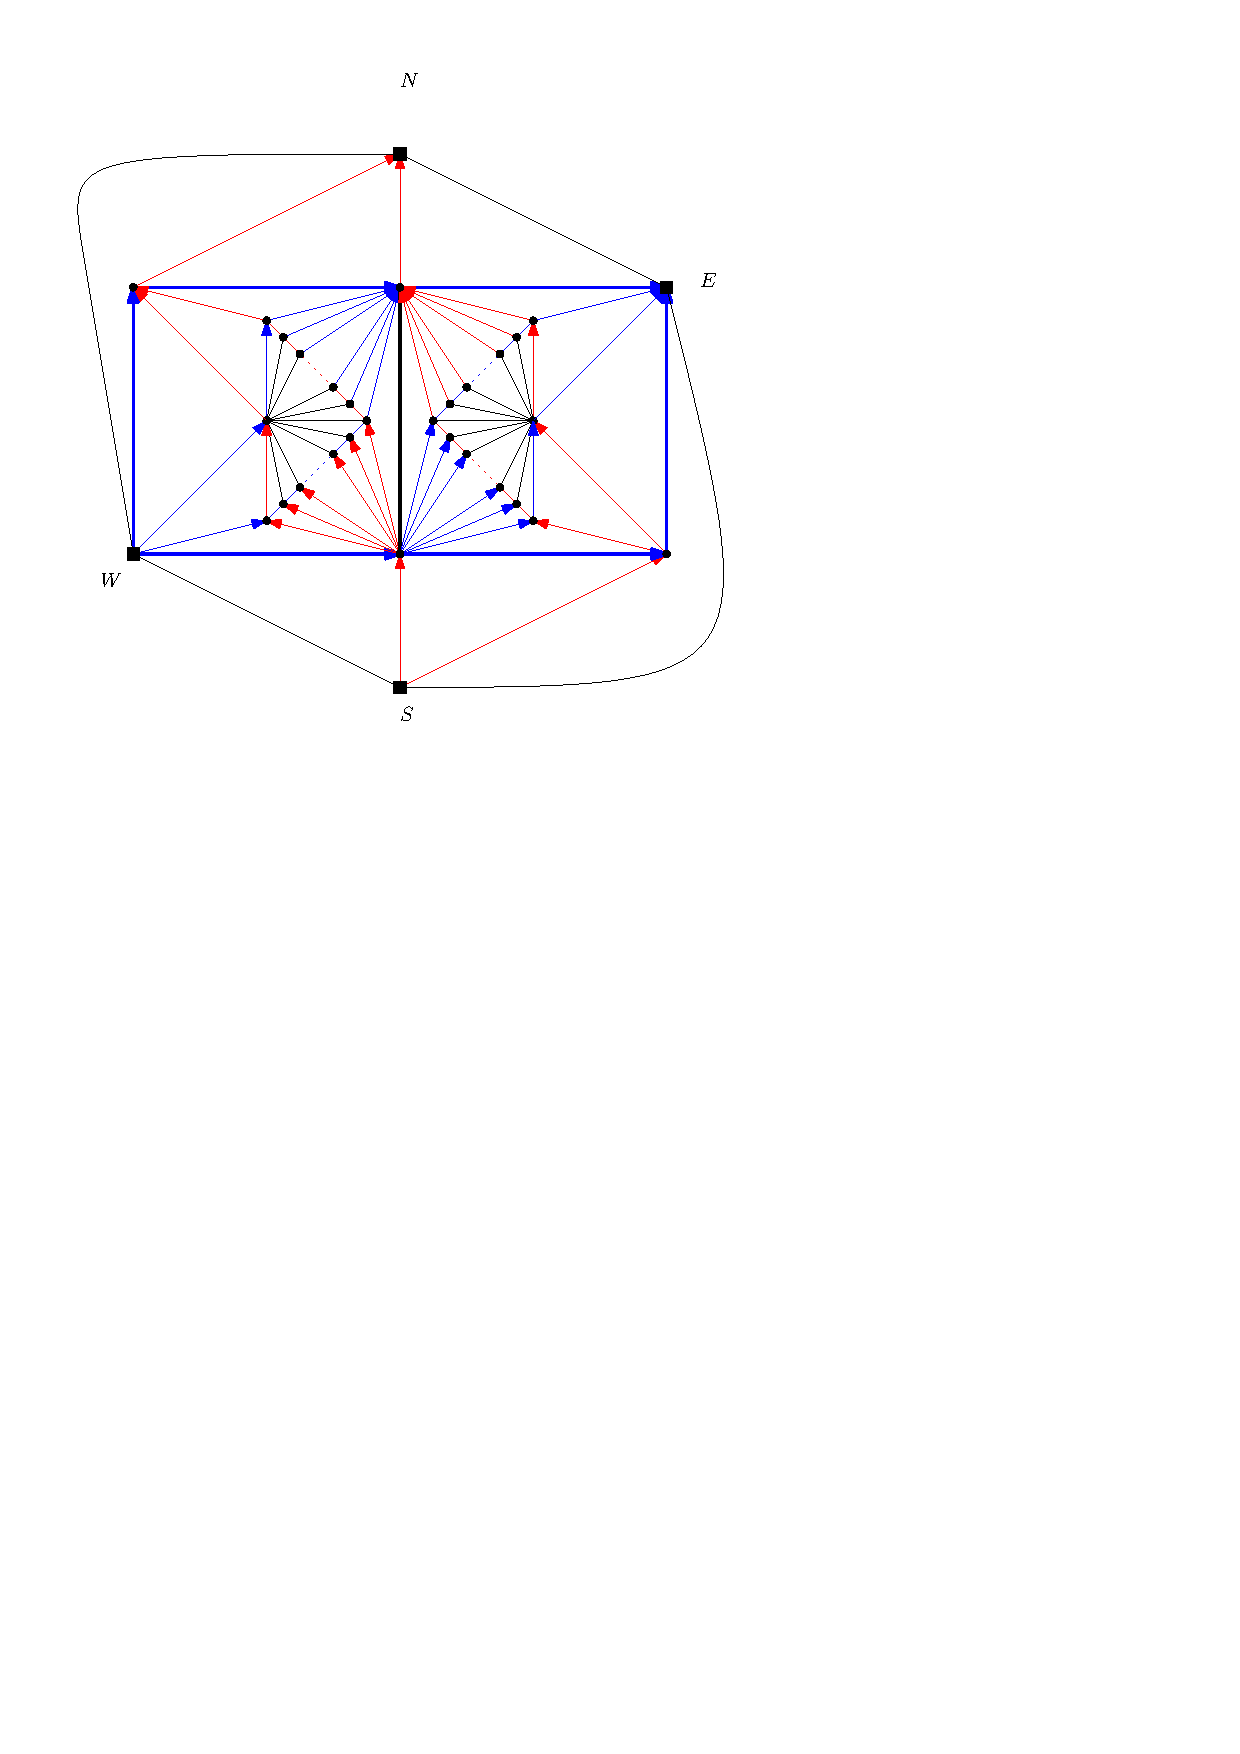
\includegraphics[width=\textwidth]{fixExtension/img/manymany3}
      \caption{Colors chosen such that there are no monochromatic triangles.}
      \label{fig:fix:manymany3}
    \end{subfigure}
    \caption{Coloring the graph.}
    \label{fig:fix:coloring}
  \end{figure}

  The result is then the graph displayed in Figure \ref{fig:fix:manymany4}. The black edges in this figure are edges that do not have a forced coloring by the above argument (Although most of them can be forced by Lemma \ref{lm:fix:fourCycleInteriorColor}).
  We focus on the centered black edge $e$, $e$ is an interior edge of both the red and blue faces drawn with dashed edges in Figure \ref{fig:fix:manymany4}. Both boundary paths of these faces are of length larger than $k$. Hence, $e$ has to be colored both red and blue to prevent that face corresponding to a $k$-sided segment occurs in the regular edge labeling. An edge can not be colored red and blue at the same time and hence $G_k$ is not $k$-sided.

  Since this proof does not depend on the value of $k$, the family $G_k$ has graphs that are not $k$-sided for any $k$.
\end{proof}


  \begin{figure}[h]
    \centering
    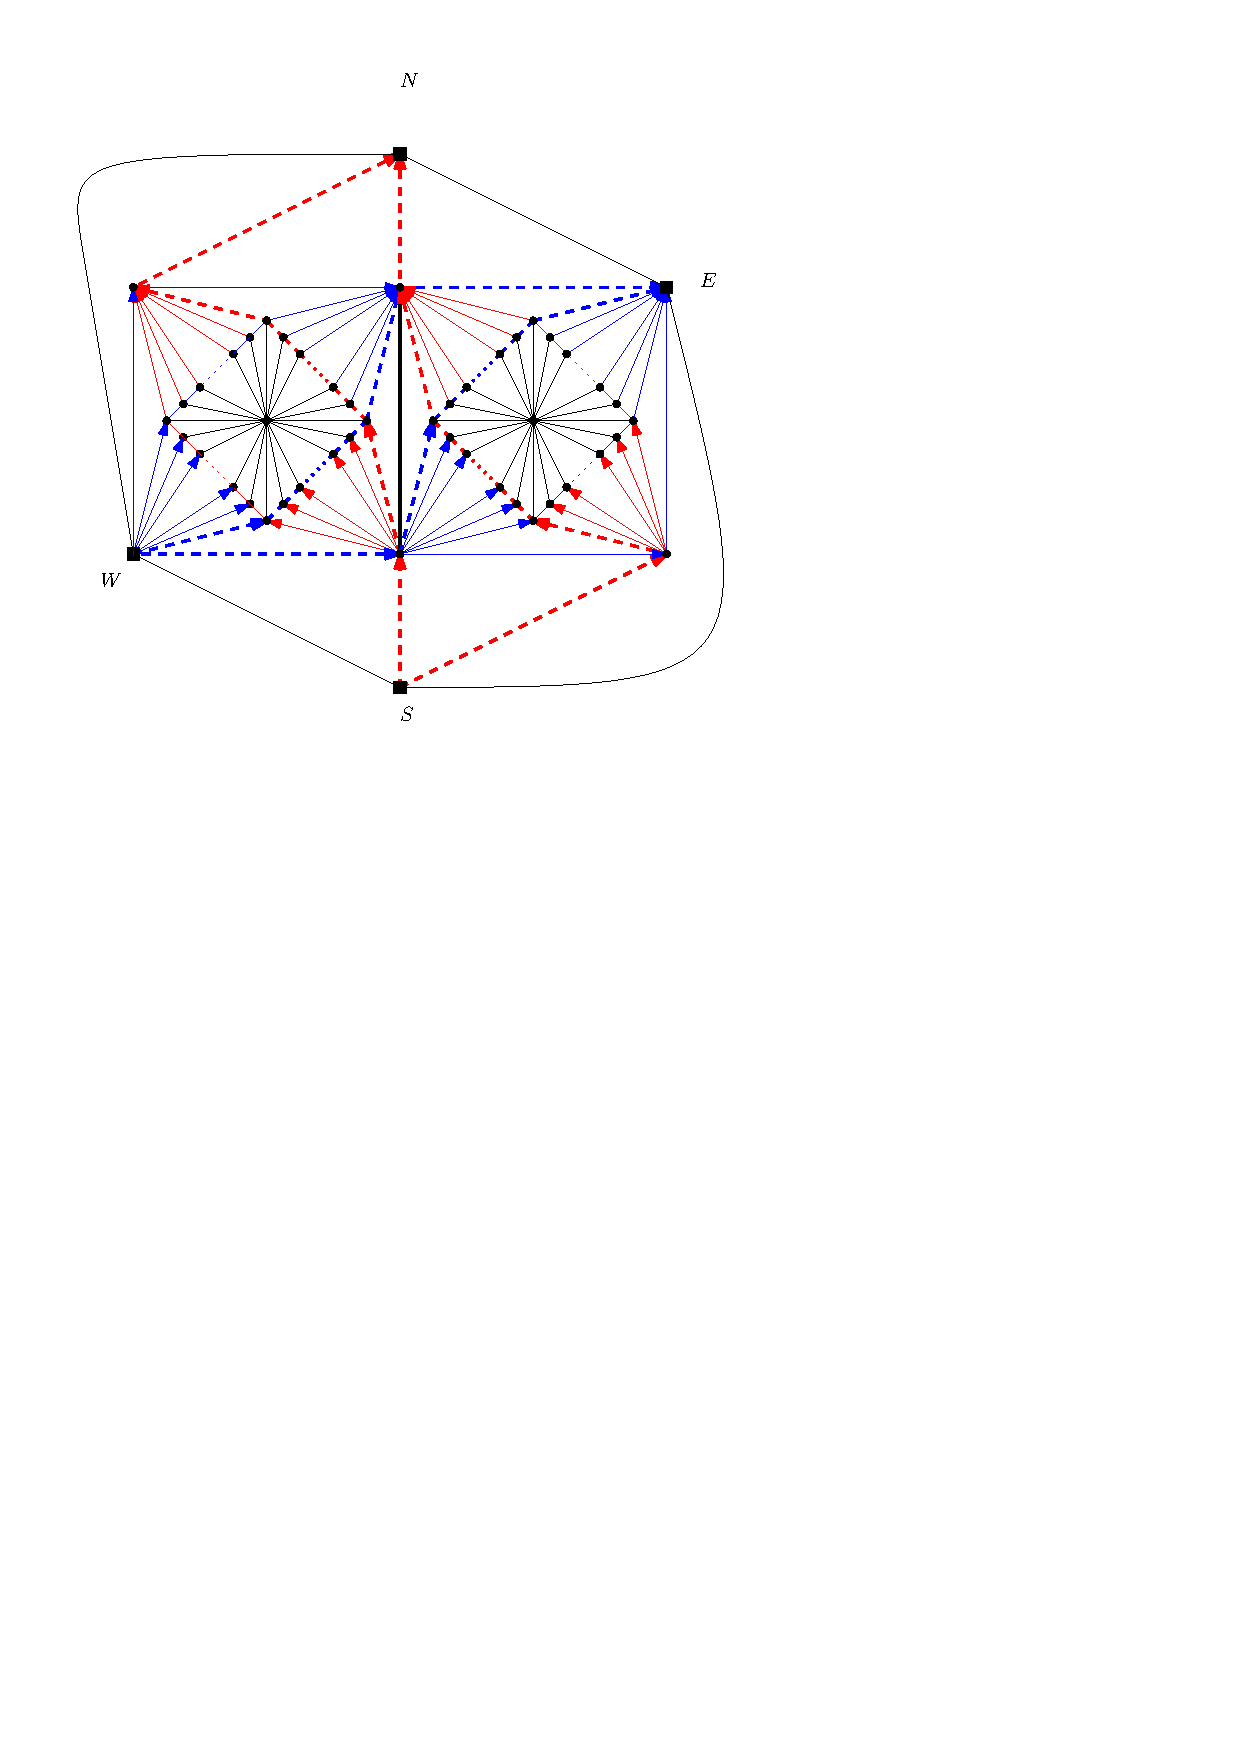
\includegraphics[scale=1]{fixExtension/img/manymany4}
    \caption{The graph after all coloring steps}
    \label{fig:fix:manymany4}
  \end{figure}
